\documentclass[12pt]{article}

\usepackage[a4paper, top=2cm, bottom=2cm, left=2.5cm, right=2.5cm]{geometry}

\usepackage{amsmath, amssymb}
\usepackage{tikz}
\usetikzlibrary{arrows.meta,positioning,fit,calc}
\usepackage{multirow}
\usepackage{array}
\usepackage{siunitx}
\usepackage{enumitem}
\usepackage{float}
\usepackage{fontspec}
\usetikzlibrary{decorations.pathmorphing}
\usepackage{pdflscape}
\usepackage{tabularx}
\usepackage{booktabs}
\usepackage{graphicx}
\usepackage{listings}
\usepackage[table]{xcolor}
\usepackage{hyperref}
\usepackage{bookmark}
\usepackage{pdfpages}


% ---------------- FONTS ----------------
% Body font
\setmainfont[
    UprightFont = Handlee-Regular.ttf,
    AutoFakeBold = 2.5
]{Handlee}

% Heading font
\newfontfamily\headingfont{PT.ttf}

% verbatim font
\setmonofont{DejaVu Sans Mono} % or Noto Sans Mono

% ---------------- HANDWRITTEN MATH ----------------
\usepackage{mathastext}
\Mathastext
\everymath{\displaystyle}

% Optional spacing tweaks (more natural look)
% \thinmuskip=2mu
% \medmuskip=2mu

% ---------------- GENERAL ----------------
\setlength{\parindent}{0pt}
\pagenumbering{gobble}
\linespread{1.2}


\newcommand{\mychapter}[2]{%
    \phantomsection
    \hypertarget{#2}{}%
    \bookmark[level=0,dest=#2]{#1}%
    \begin{center}
        {\headingfont\Huge #1}
        \par
        \vspace{4pt}
        \hrule
    \end{center}
}

\newcommand{\myquestion}[3]{%
    \phantomsection
    \hypertarget{#3}{}%
    \bookmark[level=1,dest=#3]{#1\space #2}%
    \newpage
    \noindent{\headingfont\Large #1\space #2\par}
    \vspace{4pt}
    \hrule
    \vspace{15pt}
}

\newcommand{\myanswer}[2]{
    \noindent{\headingfont\Large #1\space #2\par}
    \vspace{4pt}
    \hrule
    \vspace{15pt}
}

\newcommand{\mysubsection}[2]{
    \noindent{\headingfont\large #1\space #2\par}
    \vspace{4pt}
    \hrule
    \vspace{15pt}
}

\begin{document}

\myquestion{}{Question :}{A7K3M9Q2}

A rigid tank is divided into two compartments by a partition. One compartment contains $3$ kmol of $\mathrm{N_2}$ at $600$ kPa and the other compartment contains $7$ kmol of $\mathrm{CO_2}$ at $200$ kPa. The partition is removed, and the two gases form a homogeneous mixture at $300$ kPa.

The partial pressure of $\mathrm{N_2}$ in the mixture is

\begin{center}
\begin{tabular}{|c|c|}
\hline
\textbf{Option} & \textbf{Partial Pressure of $\mathrm{N_2}$} \\
\hline
(A) & $75$ kPa \\
\hline
(B) & $90$ kPa \\
\hline
(C) & $150$ kPa \\
\hline
(D) & $3175$ kPa \\
\hline
\end{tabular}
\end{center}

\myanswer{}{Answer :}

\textbf{\\ Mole Fraction of $\mathrm{N_2}$}

The total number of moles in the mixture is

\begin{equation*}
n_{\mathrm{total}} = n_{\mathrm{N_2}} + n_{\mathrm{CO_2}}
\end{equation*}

\begin{equation*}
n_{\mathrm{total}} = 3 + 7 = 10\ \mathrm{kmol}
\end{equation*}

Therefore, the mole fraction of $\mathrm{N_2}$ is

\begin{equation*}
y_{\mathrm{N_2}} = \frac{n_{\mathrm{N_2}}}{n_{\mathrm{total}}}
\end{equation*}

\begin{equation*}
y_{\mathrm{N_2}} = \frac{3}{10} = 0.3
\end{equation*}

\textbf{\\ Partial Pressure}

For an ideal gas mixture, the partial pressure is given by

\begin{equation*}
P_{\mathrm{N_2}} = y_{\mathrm{N_2}} P_{\mathrm{mixture}}
\end{equation*}

\begin{equation*}
P_{\mathrm{N_2}} = 0.3 \times 300
\end{equation*}

\begin{equation*}
\boxed{P_{\mathrm{N_2}} = 90\ \mathrm{kPa}}
\end{equation*}

Hence, the correct option is

\begin{equation*}
\boxed{\text{(B) }90\ \mathrm{kPa}}
\end{equation*}

\newpage
\textbf{\\ Derivation of Partial Pressure Relation}

For the entire ideal gas mixture,

\begin{equation*}
P_{\mathrm{mixture}}V=n_{\mathrm{total}}RT
\end{equation*}

For component $i$, its partial pressure is defined as the pressure exerted by component $i$ if it alone occupied the entire volume $V$ at the same temperature $T$.

Therefore,

\begin{equation*}
P_iV=n_iRT
\end{equation*}

Dividing the above two equations,

\begin{equation*}
\frac{P_iV}{P_{\mathrm{mixture}}V}
=
\frac{n_iRT}{n_{\mathrm{total}}RT}
\end{equation*}

Canceling $V$, $R$, and $T$,

\begin{equation*}
\frac{P_i}{P_{\mathrm{mixture}}}
=
\frac{n_i}{n_{\mathrm{total}}}
\end{equation*}

The mole fraction of component $i$ is defined as

\begin{equation*}
y_i=\frac{n_i}{n_{\mathrm{total}}}
\end{equation*}

Hence,

\begin{equation*}
\boxed{P_i=y_iP_{\mathrm{mixture}}}
\end{equation*}

Therefore, for nitrogen,

\begin{equation*}
\boxed{P_{\mathrm{N_2}}=y_{\mathrm{N_2}}P_{\mathrm{mixture}}}
\end{equation*}

\myquestion{}{Question :}{K7M4P2X9}

An $80$ L rigid tank contains an ideal-gas mixture of $5$ g of $\mathrm{N_2}$ and $5$ g of $\mathrm{CO_2}$ at a specified pressure and temperature. If $\mathrm{N_2}$ were separated from the mixture and stored at the mixture temperature and pressure, its volume would be

\begin{center}
\begin{tabular}{|c|c|}
\hline
\textbf{Option} & \textbf{Volume} \\
\hline
(A) & $32$ L \\
\hline
(B) & $36$ L \\
\hline
(C) & $40$ L \\
\hline
(D) & $49$ L \\
\hline
\end{tabular}
\end{center}

\myanswer{}{Answer :}

\textbf{\\ Number of moles of each gas}

For $\mathrm{N_2}$,

\begin{equation*}
n_{\mathrm{N_2}}=\frac{m_{\mathrm{N_2}}}{M_{\mathrm{N_2}}}
=\frac{5}{28}
\end{equation*}

For $\mathrm{CO_2}$,

\begin{equation*}
n_{\mathrm{CO_2}}=\frac{m_{\mathrm{CO_2}}}{M_{\mathrm{CO_2}}}
=\frac{5}{44}
\end{equation*}

The total number of moles is

\begin{equation*}
n_{\mathrm{total}}
=
\frac{5}{28}+\frac{5}{44}
\end{equation*}

\textbf{\\ Mole Fraction of $\mathrm{N_2}$}

The mole fraction of $\mathrm{N_2}$ is

\begin{equation*}
y_{\mathrm{N_2}}
=
\frac{n_{\mathrm{N_2}}}{n_{\mathrm{total}}}
\end{equation*}

\begin{equation*}
y_{\mathrm{N_2}}
=
\frac{\frac{5}{28}}
{\frac{5}{28}+\frac{5}{44}}
=
\frac{44}{72}
=
\frac{11}{18}
\end{equation*}

\textbf{\\ Volume of $\mathrm{N_2}$}

At the same temperature and pressure, the volume occupied by a component is proportional to its number of moles. Therefore,

\begin{equation*}
\frac{V_{\mathrm{N_2}}}{V_{\mathrm{mixture}}}
=
\frac{n_{\mathrm{N_2}}}{n_{\mathrm{total}}}
=
y_{\mathrm{N_2}}
\end{equation*}

Hence,

\begin{equation*}
V_{\mathrm{N_2}}
=
y_{\mathrm{N_2}}V_{\mathrm{mixture}}
\end{equation*}

\begin{equation*}
V_{\mathrm{N_2}}
=
\frac{11}{18}\times80
\end{equation*}

\begin{equation*}
\boxed{V_{\mathrm{N_2}}=48.89\ \mathrm{L}\approx49\ \mathrm{L}}
\end{equation*}

Hence, the correct option is

\begin{equation*}
\boxed{\text{(D) }49\ \mathrm{L}}
\end{equation*}






\myquestion{}{Question :}{R6T2K8P4}

An ideal-gas mixture consists of $3$ kg of Ar and $6$ kg of $\mathrm{CO_2}$ gases. The mixture is now heated at constant volume from $250$ K to $350$ K. The amount of heat transfer is

\begin{center}
\begin{tabular}{|c|c|}
\hline
\textbf{Option} & \textbf{Heat Transfer} \\
\hline
(A) & $374$ kJ \\
\hline
(B) & $436$ kJ \\
\hline
(C) & $488$ kJ \\
\hline
(D) & $525$ kJ \\
\hline
\end{tabular}
\end{center}

\myanswer{}{Answer :}

\textbf{\\ Heat Transfer at Constant Volume}

For a closed system, the first law of thermodynamics is

\begin{equation*}
Q-W=\Delta U
\end{equation*}

Since the volume is constant, the boundary work is zero:

\begin{equation*}
W=\int P\,dV=0
\end{equation*}

Therefore,

\begin{equation*}
Q=\Delta U
\end{equation*}

For an ideal-gas mixture,

\begin{equation*}
\Delta U
=
m_{\mathrm{Ar}}C_{v,\mathrm{Ar}}\Delta T
+
m_{\mathrm{CO_2}}C_{v,\mathrm{CO_2}}\Delta T
\end{equation*}

The temperature change is

\begin{equation*}
\Delta T=350-250=100\ \mathrm{K}
\end{equation*}

Using

\begin{equation*}
C_{v,\mathrm{Ar}}=0.312\ \mathrm{kJ/(kg\cdot K)}
\end{equation*}

and

\begin{equation*}
C_{v,\mathrm{CO_2}}=0.657\ \mathrm{kJ/(kg\cdot K)}
\end{equation*}

we get

\begin{equation*}
Q
=
(3)(0.312)(100)
+
(6)(0.657)(100)
\end{equation*}

\begin{equation*}
Q=93.6+394.2
\end{equation*}

\begin{equation*}
\boxed{Q=487.8\ \mathrm{kJ}\approx488\ \mathrm{kJ}}
\end{equation*}

Hence, the correct option is

\begin{equation*}
\boxed{\text{(C) }488\ \mathrm{kJ}}
\end{equation*}







\myquestion{}{Question :}{H8Q3L6R1}

An ideal-gas mixture consists of $30$ percent Helium and $70$ percent Argon gases by mass. The mixture is now expanded reversibly and adiabatically in a turbine from $400^\circ\mathrm{C}$ and $1.2$ MPa to a pressure of $200$ kPa. The mixture temperature at turbine exit is

\begin{center}
\begin{tabular}{|c|c|}
\hline
\textbf{Option} & \textbf{Temperature} \\
\hline
(A) & $195^\circ\mathrm{C}$ \\
\hline
(B) & $56^\circ\mathrm{C}$ \\
\hline
(C) & $112^\circ\mathrm{C}$ \\
\hline
(D) & $130^\circ\mathrm{C}$ \\
\hline
\end{tabular}
\end{center}

\myanswer{}{Answer :}

\textbf{\\ Specific Heat Ratio of Mixture}

Both Helium and Argon are monatomic gases. Therefore,

\begin{equation*}
\gamma_{\mathrm{He}}=\gamma_{\mathrm{Ar}}=\frac{5}{3}
\end{equation*}

Hence, the specific heat ratio of the mixture is also

\begin{equation*}
\gamma_{\mathrm{mix}}=\frac{5}{3}
\end{equation*}

\textbf{\\ Temperature-Pressure Relation}

For a reversible adiabatic process involving an ideal gas,

\begin{equation*}
\frac{T_2}{T_1}
=
\left(\frac{P_2}{P_1}\right)^{\frac{\gamma-1}{\gamma}}
\end{equation*}

The initial temperature is

\begin{equation*}
T_1=400+273=673\ \mathrm{K}
\end{equation*}

The pressure ratio is

\begin{equation*}
\frac{P_2}{P_1}
=
\frac{200}{1200}
=
\frac{1}{6}
\end{equation*}

For $\gamma=\frac{5}{3}$,

\begin{equation*}
\frac{\gamma-1}{\gamma}
=
\frac{\frac{5}{3}-1}{\frac{5}{3}}
=
\frac{2}{5}
=
0.4
\end{equation*}

Therefore,

\begin{equation*}
T_2
=
673\left(\frac{1}{6}\right)^{0.4}
\end{equation*}

\begin{equation*}
T_2\approx329\ \mathrm{K}
\end{equation*}

Converting to Celsius,

\begin{equation*}
T_2=329-273
\end{equation*}

\begin{equation*}
\boxed{T_2\approx56^\circ\mathrm{C}}
\end{equation*}

Hence, the correct option is

\begin{equation*}
\boxed{\text{(B) }56^\circ\mathrm{C}}
\end{equation*}

\myquestion{}{Question :}{K7M4P2Q9}

A piston-cylinder device contains an ideal-gas mixture of 3 kmol of He gas and 7 kmol of Ar gas at $50^\circ\mathrm{C}$ and $400\ \mathrm{kPa}$. The gas expands at constant pressure until its volume doubles. The amount of heat transfer to the gas mixture is

\begin{equation*}
\mathrm{(A)}\ 6.2\ \mathrm{MJ}
\qquad
\mathrm{(B)}\ 4.2\ \mathrm{MJ}
\qquad
\mathrm{(C)}\ 27\ \mathrm{MJ}
\qquad
\mathrm{(D)}\ 67\ \mathrm{MJ}
\end{equation*}

\myanswer{}{Answer :}

For both He and Ar, which are monatomic ideal gases,

\begin{equation*}
C_p=\frac{5}{2}R
\end{equation*}

Since the pressure is constant and the gas mixture behaves as an ideal gas,

\begin{equation*}
PV=nRT
\end{equation*}

Therefore, at constant pressure,

\begin{equation*}
V\propto T
\end{equation*}

Since the volume doubles,

\begin{equation*}
T_2=2T_1
\end{equation*}

The initial temperature is

\begin{equation*}
T_1=50+273.15=323.15\ \mathrm{K}
\end{equation*}

Hence,

\begin{equation*}
\Delta T=T_2-T_1=T_1=323.15\ \mathrm{K}
\end{equation*}

The total amount of gas is

\begin{equation*}
n=3+7=10\ \mathrm{kmol}
\end{equation*}

For a constant-pressure process, the heat transfer is

\begin{equation*}
Q=nC_p\Delta T
\end{equation*}

Substituting the values,

\begin{equation*}
Q=(10)\left(\frac{5}{2}\times8.314\right)(323.15)
\end{equation*}

\begin{equation*}
Q=67180\ \mathrm{kJ}
\end{equation*}

\begin{equation*}
Q\approx67.18\ \mathrm{MJ}
\end{equation*}

Therefore,

\begin{equation*}
\boxed{Q\approx67\ \mathrm{MJ}}
\end{equation*}

Hence, the correct answer is

\begin{equation*}
\boxed{\mathrm{(D)}\ 67\ \mathrm{MJ}}
\end{equation*}

\newpage

\begin{center}
\Large{Alternate Method\\}  
\end{center}
\hrule

\vspace*{0.2cm}
The mole fractions of He and Ar in the mixture are

\begin{equation*}
y_{\mathrm{He}}=\frac{3}{3+7}=0.3
\end{equation*}

\begin{equation*}
y_{\mathrm{Ar}}=\frac{7}{3+7}=0.7
\end{equation*}

For monatomic ideal gases, the molar specific heat at constant pressure is

\begin{equation*}
C_{p,\mathrm{He}}=20.785\ \mathrm{kJ/(kmol\cdot K)}
\end{equation*}

\begin{equation*}
C_{p,\mathrm{Ar}}=20.785\ \mathrm{kJ/(kmol\cdot K)}
\end{equation*}

The specific heat of the gas mixture is obtained from the mole-fraction relation

\begin{equation*}
C_{p,\mathrm{mix}}
=
y_{\mathrm{He}}C_{p,\mathrm{He}}
+
y_{\mathrm{Ar}}C_{p,\mathrm{Ar}}
\end{equation*}

Substituting the values,

\begin{equation*}
C_{p,\mathrm{mix}}
=
(0.3)(20.785)+(0.7)(20.785)
\end{equation*}

\begin{equation*}
C_{p,\mathrm{mix}}
=
20.785\ \mathrm{kJ/(kmol\cdot K)}
\end{equation*}

Since the pressure is constant and the gas behaves ideally,

\begin{equation*}
V\propto T
\end{equation*}

Since the volume doubles,

\begin{equation*}
T_2=2T_1
\end{equation*}

The initial temperature is

\begin{equation*}
T_1=50+273.15=323.15\ \mathrm{K}
\end{equation*}

Therefore,

\begin{equation*}
\Delta T=T_2-T_1=323.15\ \mathrm{K}
\end{equation*}

The total amount of gas is

\begin{equation*}
n=3+7=10\ \mathrm{kmol}
\end{equation*}

For a constant-pressure process, the heat transfer is

\begin{equation*}
Q=nC_{p,\mathrm{mix}}\Delta T
\end{equation*}

Substituting the values,

\begin{equation*}
Q=(10)(20.785)(323.15)
\end{equation*}

\begin{equation*}
Q=67180\ \mathrm{kJ}
\end{equation*}

\begin{equation*}
Q\approx67.18\ \mathrm{MJ}
\end{equation*}

Therefore,

\begin{equation*}
\boxed{Q\approx67\ \mathrm{MJ}}
\end{equation*}

Hence, the correct answer is

\begin{equation*}
\boxed{\mathrm{(D)}\ 67\ \mathrm{MJ}}
\end{equation*}






















\myquestion{}{Question :}{Q6A7B2K9}

The temperature $t$ on a thermometric scale is defined in terms of a property $K$ by the relation

\begin{equation*}
t=a\ln K+b
\end{equation*}

where $a$ and $b$ are constants. The values of $K$ are found to be $1.83$ and $6.78$ at the ice point and the steam point, the temperatures of which are assigned the numbers $0$ and $100$, respectively. Determine the temperature corresponding to a reading of $K=2.42$ on the thermometer.

\myanswer{}{Answer :}

The thermometric relation is

\begin{equation*}
t=a\ln K+b
\end{equation*}

At the ice point, $t=0$ and $K=1.83$.

\begin{equation*}
0=a\ln(1.83)+b
\end{equation*}

Therefore,

\begin{equation*}
b=-a\ln(1.83)
\end{equation*}

At the steam point, $t=100$ and $K=6.78$.

\begin{equation*}
100=a\ln(6.78)+b
\end{equation*}

Substituting the value of $b$,

\begin{equation*}
100=a\ln(6.78)-a\ln(1.83)
\end{equation*}

\begin{equation*}
100=a\ln\left(\frac{6.78}{1.83}\right)
\end{equation*}

Hence,

\begin{equation*}
a=\frac{100}{\ln(6.78/1.83)}
\end{equation*}

For $K=2.42$,

\begin{equation*}
t=a\ln(2.42)+b
\end{equation*}

Using $b=-a\ln(1.83)$,

\begin{equation*}
t=a\left[\ln(2.42)-\ln(1.83)\right]
\end{equation*}

\begin{equation*}
t=a\ln\left(\frac{2.42}{1.83}\right)
\end{equation*}

Substituting the value of $a$,

\begin{equation*}
t=
100\frac{\ln(2.42/1.83)}
{\ln(6.78/1.83)}
\end{equation*}

\begin{equation*}
t=21.34^\circ
\end{equation*}

Since the answer is required as an integer,

\begin{equation*}
\boxed{t=21^\circ}
\end{equation*}






















\myquestion{}{Question :}{R8K3M6P1}

A new scale N of temperature is divided in such a way that the freezing point of ice is $100^\circ\mathrm{N}$ and the boiling point is $400^\circ\mathrm{N}$. What is the temperature reading on this new scale when the temperature is $150^\circ\mathrm{C}$? At what temperature would both the Celsius and the new temperature scale readings be the same? (Answer in integer.)

\myanswer{}{Answer :}

The relation between the Celsius scale and the new scale is linear.

At the freezing point,

\begin{equation*}
0^\circ\mathrm{C}=100^\circ\mathrm{N}
\end{equation*}

At the boiling point,

\begin{equation*}
100^\circ\mathrm{C}=400^\circ\mathrm{N}
\end{equation*}

Therefore, the change of $300^\circ\mathrm{N}$ corresponds to a change of $100^\circ\mathrm{C}$.

Hence,

\begin{equation*}
\frac{N-100}{C-0}=\frac{400-100}{100-0}
\end{equation*}

\begin{equation*}
N-100=3C
\end{equation*}

For $C=150^\circ\mathrm{C}$,

\begin{equation*}
N=100+3(150)
\end{equation*}

\begin{equation*}
N=550^\circ\mathrm{N}
\end{equation*}

Now, let the temperature at which the two scale readings are equal be $T$.

Thus,

\begin{equation*}
N=C=T
\end{equation*}

Using the relation between the two scales,

\begin{equation*}
T=100+3T
\end{equation*}

\begin{equation*}
2T=-100
\end{equation*}

\begin{equation*}
T=-50^\circ\mathrm{C}
\end{equation*}
























\myquestion{}{Question :}{H6P3R8K2}

Match List-I with List-II and select the correct answer using the codes given below the lists.

\textbf{List-I (Parameter)}

\begin{equation*}
\mathrm{A.}\ \text{Volume}
\end{equation*}

\begin{equation*}
\mathrm{B.}\ \text{Density}
\end{equation*}

\begin{equation*}
\mathrm{C.}\ \text{Pressure}
\end{equation*}

\begin{equation*}
\mathrm{D.}\ \text{Work}
\end{equation*}

\textbf{List-II (Property)}

\begin{equation*}
1.\ \text{Path function}
\end{equation*}

\begin{equation*}
2.\ \text{Intensive property}
\end{equation*}

\begin{equation*}
3.\ \text{Extensive property}
\end{equation*}

\begin{equation*}
4.\ \text{Point function}
\end{equation*}

\myanswer{}{Answer :}

Volume is an extensive property because it depends on the amount of matter in the system.

\begin{equation*}
\mathrm{A}\longrightarrow3
\end{equation*}

Density is an intensive property because it does not depend on the amount of matter.

\begin{equation*}
\mathrm{B}\longrightarrow2
\end{equation*}

Pressure is an intensive property because it does not depend on the amount of matter.

\begin{equation*}
\mathrm{C}\longrightarrow2
\end{equation*}

Work is a path function because its value depends on the path followed during the process.

\begin{equation*}
\mathrm{D}\longrightarrow1
\end{equation*}

Therefore, the correct matching is

\begin{equation*}
\boxed{\mathrm{A}-3,\quad B-2,\quad C-2,\quad D-1}
\end{equation*}






































\myquestion{}{Question :}{T4M8K2P6}

Consider the following statements:

A real gas obeys perfect gas law at very

\begin{equation*}
1.\ \text{High temperatures}
\end{equation*}

\begin{equation*}
2.\ \text{High pressures}
\end{equation*}

\begin{equation*}
3.\ \text{Low pressures}
\end{equation*}

Which of these statements is/are correct?

\begin{equation*}
\mathrm{(A)}\ 1\ \text{alone}
\qquad
\mathrm{(B)}\ 1\ \text{and}\ 3
\end{equation*}

\begin{equation*}
\mathrm{(C)}\ 2\ \text{alone}
\qquad
\mathrm{(D)}\ 3\ \text{alone}
\end{equation*}

\myanswer{}{Answer :}

A real gas approaches ideal-gas behavior when the intermolecular forces and the volume occupied by the molecules become negligible compared with the overall volume of the gas.

At high temperatures, the kinetic energy of the molecules is high, reducing the relative effect of intermolecular attractive forces.

\begin{equation*}
\text{High temperature}\longrightarrow\text{Ideal-gas behavior}
\end{equation*}

At low pressures, the molecules are far apart and their intermolecular forces and molecular volume become negligible.

\begin{equation*}
\text{Low pressure}\longrightarrow\text{Ideal-gas behavior}
\end{equation*}

At high pressures, the molecules are brought closer together, so intermolecular forces and molecular volume become significant. Hence, a real gas does not closely obey the perfect-gas law at high pressures.

Therefore, statements $1$ and $3$ are correct.

\begin{equation*}
\boxed{\mathrm{(B)}\ 1\ \text{and}\ 3}
\end{equation*}























\myquestion{}{Question :}{B6K2P9R4}

The volume $V$ versus temperature $T$ graphs for a certain amount of a perfect ideal gas at two pressures $P_1$ and $P_2$ are shown in the figure. Which is greater, $P_1$ or $P_2$?

\begin{figure}[H] % h = here, t = top, b = bottom, p = page of floats
    \centering
    \fbox{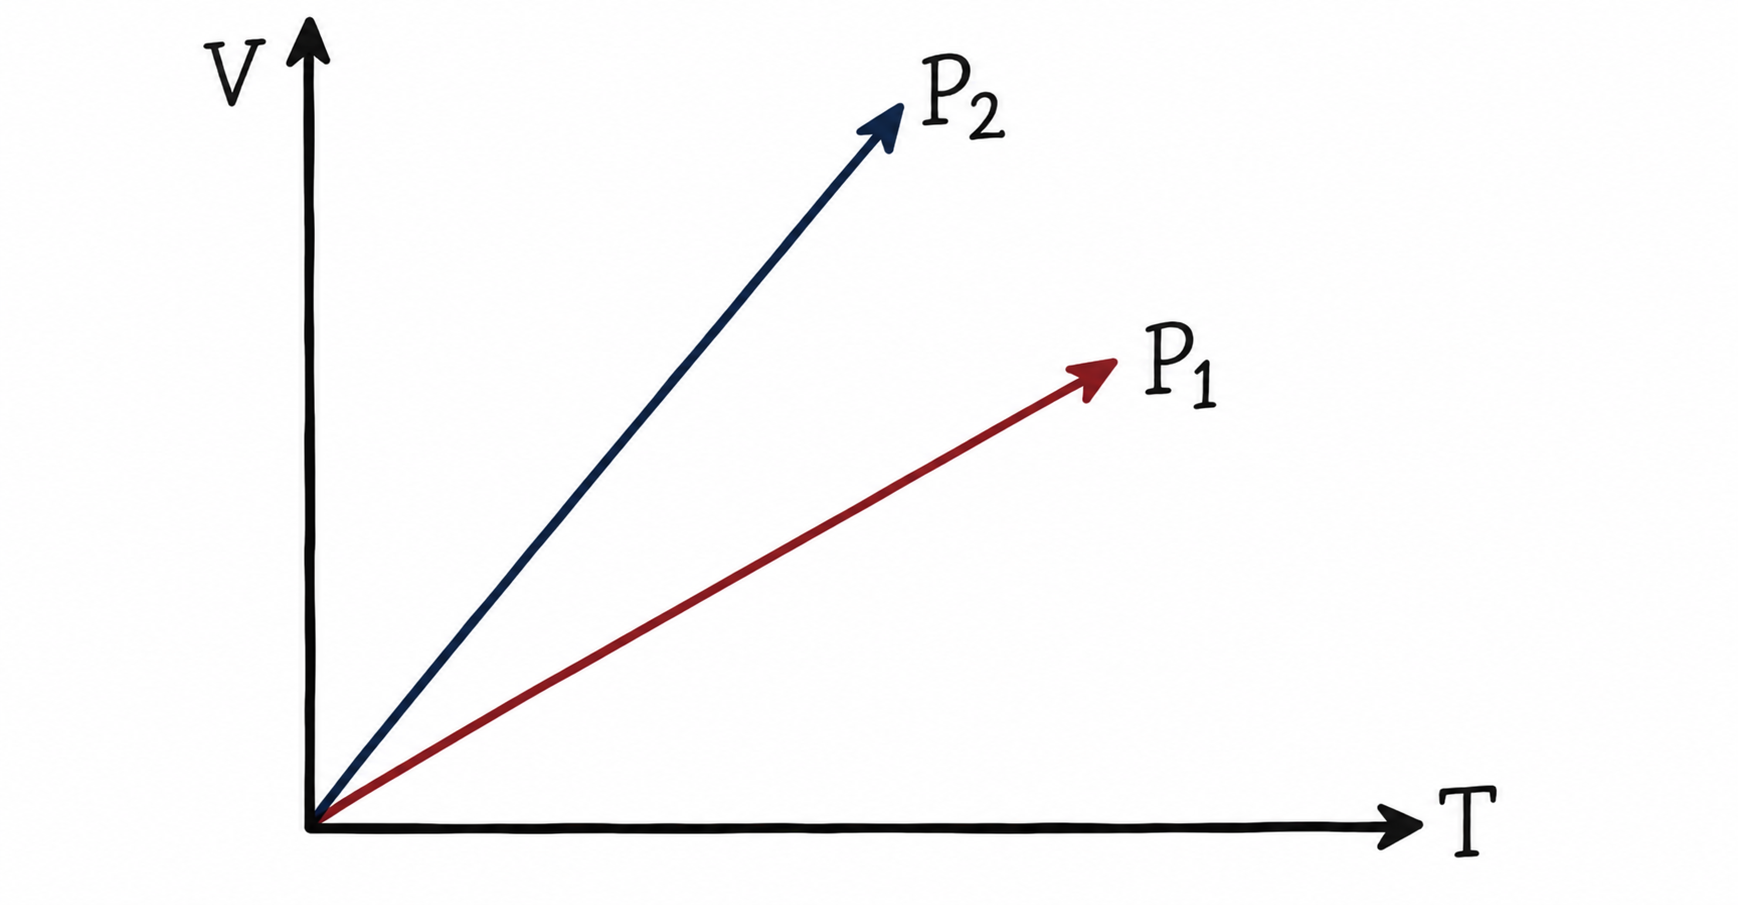
\includegraphics[width=0.45\textwidth]{../2. Figures/Figure : 8.png}}
    \label{fig:myimage}
\end{figure}

\myanswer{}{Answer :}

For a perfect ideal gas,

\begin{equation*}
PV=nRT
\end{equation*}

For a fixed amount of gas,

\begin{equation*}
V=\frac{nR}{P}T
\end{equation*}

Comparing this with the equation of a straight line,

\begin{equation*}
V=\left(\frac{nR}{P}\right)T
\end{equation*}

Therefore, the slope of the $V$ versus $T$ graph is

\begin{equation*}
\text{Slope}=\frac{nR}{P}
\end{equation*}

Thus, the slope is inversely proportional to pressure.

From the graph, the line corresponding to $P_2$ has a greater slope than the line corresponding to $P_1$.

Therefore,

\begin{equation*}
\frac{nR}{P_2}>\frac{nR}{P_1}
\end{equation*}

Hence,

\begin{equation*}
P_2<P_1
\end{equation*}

Therefore, the correct answer is

\begin{equation*}
\boxed{\mathrm{(A)}\ P_2<P_1}
\end{equation*}





























\end{document}